% coding:utf-8

%----------------------------------------
%FOSAPHY, a LaTeX-Code for a summary of modern control theory
%Copyright (C) 2015, Mario Felder & Michi Fallegger

%This program is free software; you can redistribute it and/or
%modify it under the terms of the GNU General Public License
%as published by the Free Software Foundation; either version 2
%of the License, or (at your option) any later version.

%This program is distributed in the hope that it will be useful,
%but WITHOUT ANY WARRANTY; without even the implied warranty of
%MERCHANTABILITY or FITNESS FOR A PARTICULAR PURPOSE.  See the
%GNU General Public License for more details.
%----------------------------------------

\chapter{Digitale Regelung}

\section{Schematische Darstellung}
\begin{center}
	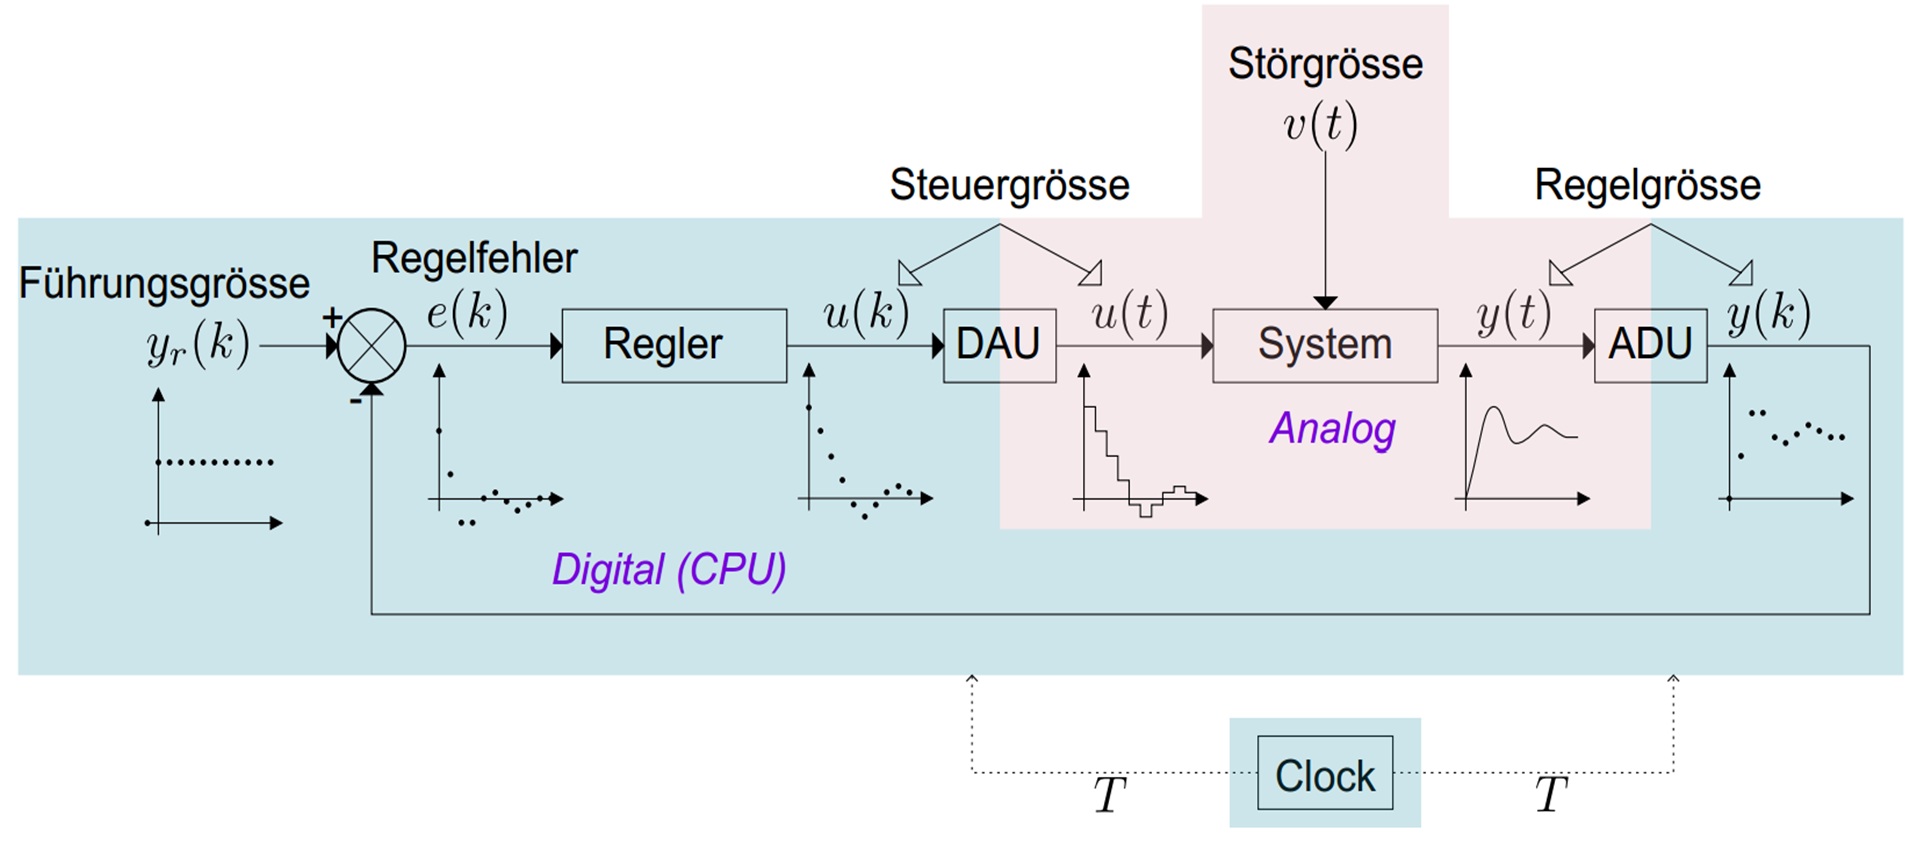
\includegraphics[scale = 0.3]{images/schematische_darstellung.png}
\end{center}
\[
	G(s)=\frac{Y(s)}{U(s)}\\ \rightarrow \\ H(z)=\frac{Y(z)}{U(z)} \\ \\
\]

\section{Direkter/Indirekter Regler}
\begin{center}
	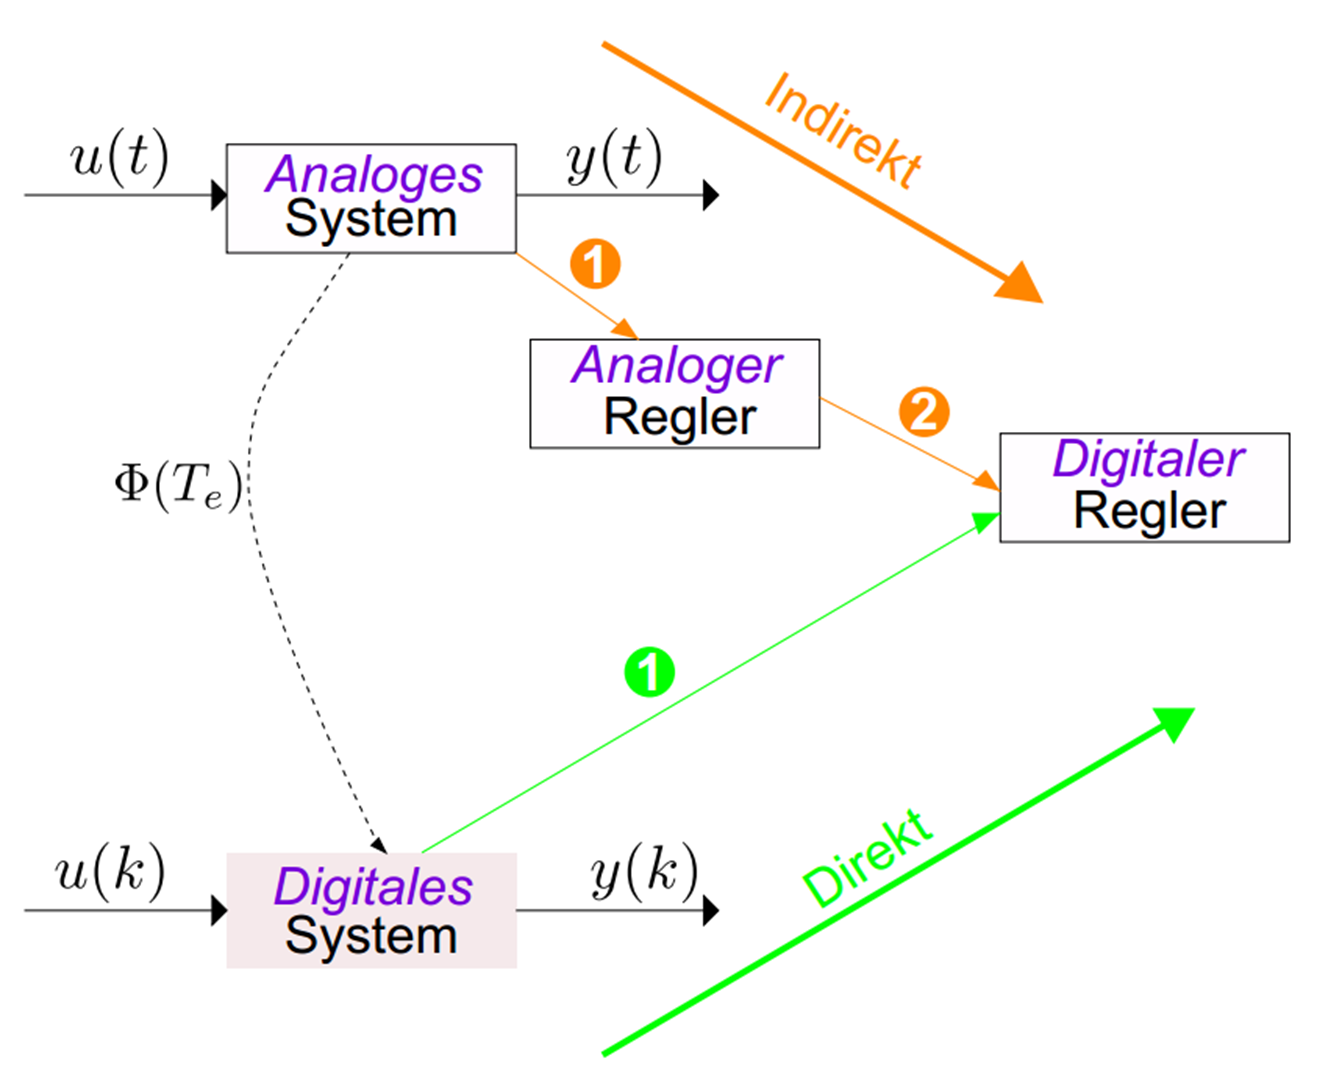
\includegraphics[scale = 0.25]{images/direkter_indirekter.png}
\end{center}

\section{Digitaler PID}
Wir haben:
\[
	u(t)=u_{k,a}(e(t))+u_{i,a}(e(t))+u_{d,a}(e(t))
\]
Wir wollen:
\[
	u(k)=u_{k,a}(e(k))+u_{i,a}(e(k))+u_{d,a}(e(k))
\]
\subsection{I Anteil}
Implementierbare Differenzgleichungen für I-Anteil:\\
Rückwärts-Rechteckregel:
\[
	u_{i,d,r}(e(k)))=u_{i,d,r}(e(k-1))+\frac{K_a}{T_{i,a}}e(k)\cdot T
\]
Trapezregel:
\[
	u_{i,d,r}(e(k)))=u_{i,d,r}(e(k-1))+\frac{K_a}{T_{i,a}}\cdot \frac{e(k)+e(k-1)}{2}\cdot T
\]
\subsection{D Anteil}
\[
	u_{d,d}(e(k))=K_aT_{d,a} \cdot \frac{e(k)-e(k-1)}{T}
\]
\subsection{Antireset-Windup}
\[
	u_{nosat}(k)= u_p(k)+u_i(k-1)+u(d)	
\]
\[
	if( u_{nosat}(k)>u_{sat,max})\\{u(k) =  u_{sat,max} } \\ \\ \\
\]
\[
	else if(u_{nosat}(k)<u_{sat,min})
\]
\[
	{u(k) =  u_{sat,min} } \\ \\
\]
\[
	u_i(k)= u_i(k-1)+K_a\frac{T}{Ti}\cdot\frac{e(k)+e(k-1)}{2}+\frac{T}{T_r}(u(k)-u(k)_{nosat})
\]
\\
\section{z-Transformation}
\begin{center}
	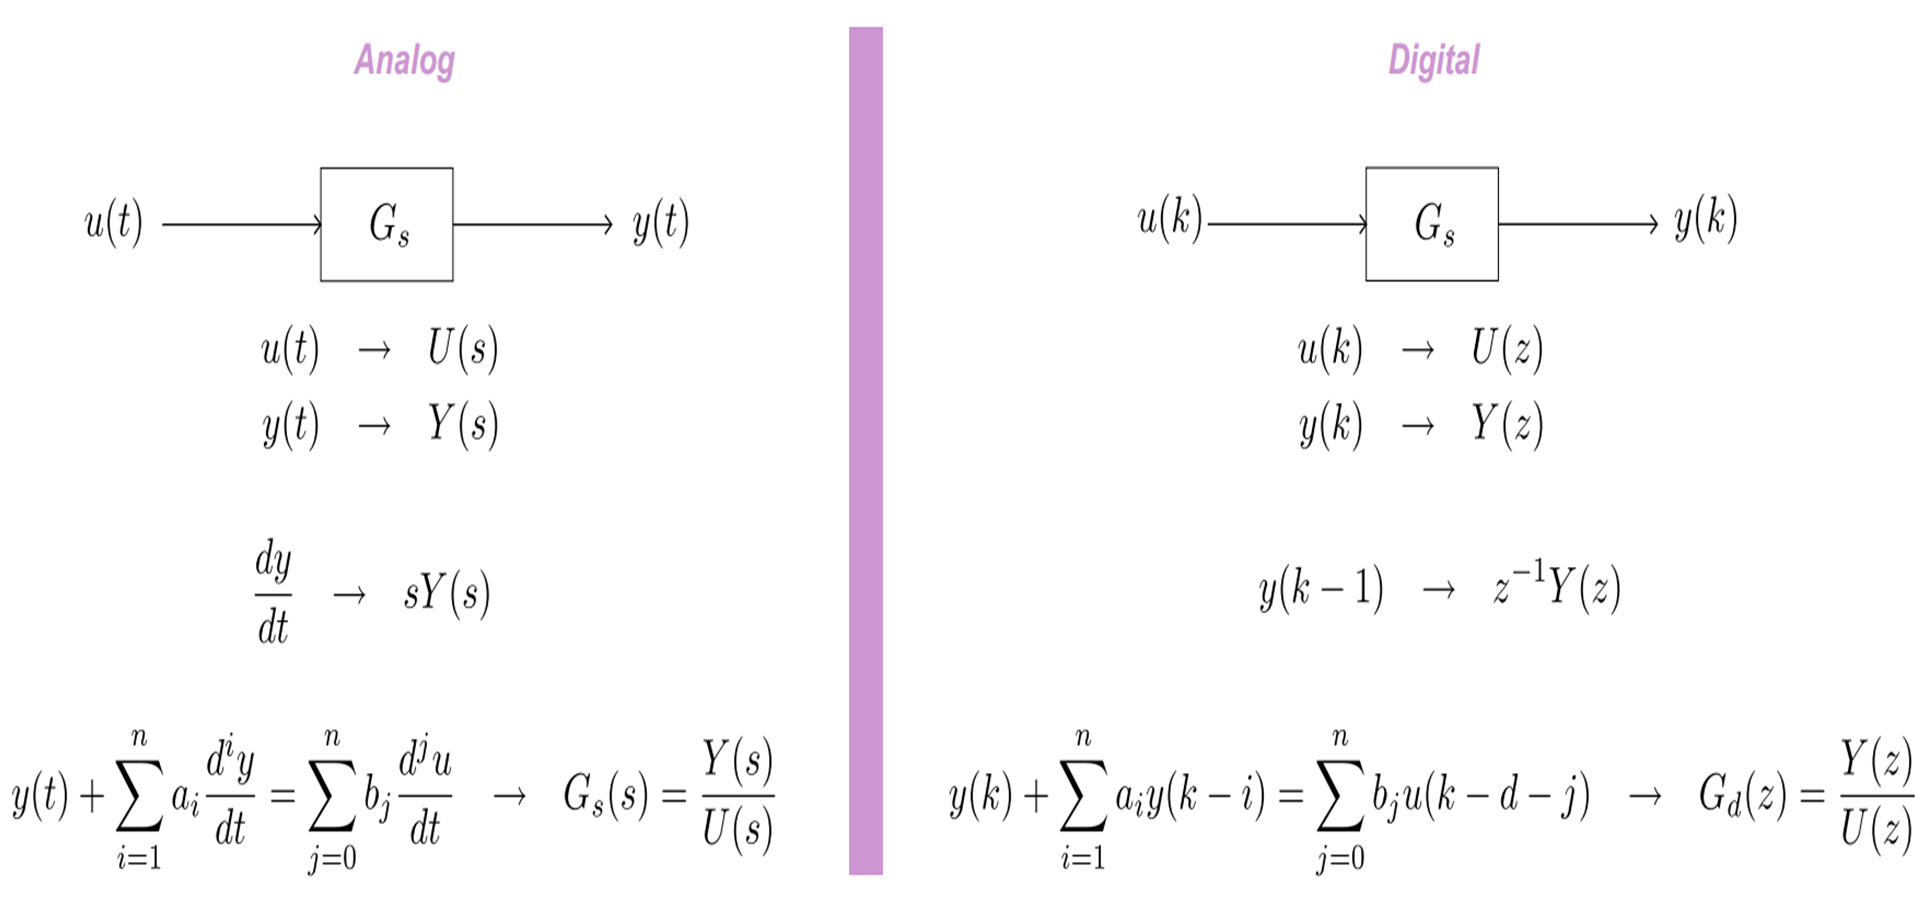
\includegraphics[scale = 0.25]{images/z_transf.png}
\end{center}
\subsection{Antworten}
Impulsantwort:
\[
	Z\left\lbrace I_i(k)\right\rbrace  =z^{-l}\\
	\\\begin{cases}1&\text{1 if k $0$ l}\\2&\text{0 if k $\neq$ l}\end{cases} \\ \\
\]
Sprungantwort:
\[
	Z\left\lbrace I_i(k)\right\rbrace  =\sum_{i=l}^{\infty}z^{-i}=u^{-l}\frac{z}{z-1}
	\\\begin{cases}1&\text{1 if k $\geq$ l}\\2&\text{0 if k $<$ l}\end{cases} \\ \\
\]

